\documentclass[11pt,titlepage,dvipsnames,table,xcdraw,english]{article}
%!TEX root=./latex-dissertation.tex
%% ODER: format ==         = "\mathrel{==}"
%% ODER: format /=         = "\neq "
%
%
\makeatletter
\@ifundefined{lhs2tex.lhs2tex.sty.read}%
  {\@namedef{lhs2tex.lhs2tex.sty.read}{}%
   \newcommand\SkipToFmtEnd{}%
   \newcommand\EndFmtInput{}%
   \long\def\SkipToFmtEnd#1\EndFmtInput{}%
  }\SkipToFmtEnd

\newcommand\ReadOnlyOnce[1]{\@ifundefined{#1}{\@namedef{#1}{}}\SkipToFmtEnd}
\usepackage{amstext}
\usepackage{amssymb}
\usepackage{stmaryrd}
\DeclareFontFamily{OT1}{cmtex}{}
\DeclareFontShape{OT1}{cmtex}{m}{n}
  {<5><6><7><8>cmtex8
   <9>cmtex9
   <10><10.95><12><14.4><17.28><20.74><24.88>cmtex10}{}
\DeclareFontShape{OT1}{cmtex}{m}{it}
  {<-> ssub * cmtt/m/it}{}
\newcommand{\texfamily}{\fontfamily{cmtex}\selectfont}
\DeclareFontShape{OT1}{cmtt}{bx}{n}
  {<5><6><7><8>cmtt8
   <9>cmbtt9
   <10><10.95><12><14.4><17.28><20.74><24.88>cmbtt10}{}
\DeclareFontShape{OT1}{cmtex}{bx}{n}
  {<-> ssub * cmtt/bx/n}{}
\newcommand{\tex}[1]{\text{\texfamily#1}}	% NEU

\newcommand{\Sp}{\hskip.33334em\relax}


\newcommand{\Conid}[1]{\mathit{#1}}
\newcommand{\Varid}[1]{\mathit{#1}}
\newcommand{\anonymous}{\kern0.06em \vbox{\hrule\@width.5em}}
\newcommand{\plus}{\mathbin{+\!\!\!+}}
\newcommand{\bind}{\mathbin{>\!\!\!>\mkern-6.7mu=}}
\newcommand{\rbind}{\mathbin{=\mkern-6.7mu<\!\!\!<}}% suggested by Neil Mitchell
\newcommand{\sequ}{\mathbin{>\!\!\!>}}
\renewcommand{\leq}{\leqslant}
\renewcommand{\geq}{\geqslant}
\usepackage{polytable}

%mathindent has to be defined
\@ifundefined{mathindent}%
  {\newdimen\mathindent\mathindent\leftmargini}%
  {}%

\def\resethooks{%
  \global\let\SaveRestoreHook\empty
  \global\let\ColumnHook\empty}
\newcommand*{\savecolumns}[1][default]%
  {\g@addto@macro\SaveRestoreHook{\savecolumns[#1]}}
\newcommand*{\restorecolumns}[1][default]%
  {\g@addto@macro\SaveRestoreHook{\restorecolumns[#1]}}
\newcommand*{\aligncolumn}[2]%
  {\g@addto@macro\ColumnHook{\column{#1}{#2}}}

\resethooks

\newcommand{\onelinecommentchars}{\quad-{}- }
\newcommand{\commentbeginchars}{\enskip\{-}
\newcommand{\commentendchars}{-\}\enskip}

\newcommand{\visiblecomments}{%
  \let\onelinecomment=\onelinecommentchars
  \let\commentbegin=\commentbeginchars
  \let\commentend=\commentendchars}

\newcommand{\invisiblecomments}{%
  \let\onelinecomment=\empty
  \let\commentbegin=\empty
  \let\commentend=\empty}

\visiblecomments

\newlength{\blanklineskip}
\setlength{\blanklineskip}{0.66084ex}

\newcommand{\hsindent}[1]{\quad}% default is fixed indentation
\let\hspre\empty
\let\hspost\empty
\newcommand{\NB}{\textbf{NB}}
\newcommand{\Todo}[1]{$\langle$\textbf{To do:}~#1$\rangle$}

\EndFmtInput
\makeatother
%
%
%
%
%
%
% This package provides two environments suitable to take the place
% of hscode, called "plainhscode" and "arrayhscode". 
%
% The plain environment surrounds each code block by vertical space,
% and it uses \abovedisplayskip and \belowdisplayskip to get spacing
% similar to formulas. Note that if these dimensions are changed,
% the spacing around displayed math formulas changes as well.
% All code is indented using \leftskip.
%
% Changed 19.08.2004 to reflect changes in colorcode. Should work with
% CodeGroup.sty.
%
\ReadOnlyOnce{polycode.fmt}%
\makeatletter

\newcommand{\hsnewpar}[1]%
  {{\parskip=0pt\parindent=0pt\par\vskip #1\noindent}}

% can be used, for instance, to redefine the code size, by setting the
% command to \small or something alike
\newcommand{\hscodestyle}{}

% The command \sethscode can be used to switch the code formatting
% behaviour by mapping the hscode environment in the subst directive
% to a new LaTeX environment.

\newcommand{\sethscode}[1]%
  {\expandafter\let\expandafter\hscode\csname #1\endcsname
   \expandafter\let\expandafter\endhscode\csname end#1\endcsname}

% "compatibility" mode restores the non-polycode.fmt layout.

\newenvironment{compathscode}%
  {\par\noindent
   \advance\leftskip\mathindent
   \hscodestyle
   \let\\=\@normalcr
   \let\hspre\(\let\hspost\)%
   \pboxed}%
  {\endpboxed\)%
   \par\noindent
   \ignorespacesafterend}

\newcommand{\compaths}{\sethscode{compathscode}}

% "plain" mode is the proposed default.
% It should now work with \centering.
% This required some changes. The old version
% is still available for reference as oldplainhscode.

\newenvironment{plainhscode}%
  {\hsnewpar\abovedisplayskip
   \advance\leftskip\mathindent
   \hscodestyle
   \let\hspre\(\let\hspost\)%
   \pboxed}%
  {\endpboxed%
   \hsnewpar\belowdisplayskip
   \ignorespacesafterend}

\newenvironment{oldplainhscode}%
  {\hsnewpar\abovedisplayskip
   \advance\leftskip\mathindent
   \hscodestyle
   \let\\=\@normalcr
   \(\pboxed}%
  {\endpboxed\)%
   \hsnewpar\belowdisplayskip
   \ignorespacesafterend}

% Here, we make plainhscode the default environment.

\newcommand{\plainhs}{\sethscode{plainhscode}}
\newcommand{\oldplainhs}{\sethscode{oldplainhscode}}
\plainhs

% The arrayhscode is like plain, but makes use of polytable's
% parray environment which disallows page breaks in code blocks.

\newenvironment{arrayhscode}%
  {\hsnewpar\abovedisplayskip
   \advance\leftskip\mathindent
   \hscodestyle
   \let\\=\@normalcr
   \(\parray}%
  {\endparray\)%
   \hsnewpar\belowdisplayskip
   \ignorespacesafterend}

\newcommand{\arrayhs}{\sethscode{arrayhscode}}

% The mathhscode environment also makes use of polytable's parray 
% environment. It is supposed to be used only inside math mode 
% (I used it to typeset the type rules in my thesis).

\newenvironment{mathhscode}%
  {\parray}{\endparray}

\newcommand{\mathhs}{\sethscode{mathhscode}}

% texths is similar to mathhs, but works in text mode.

\newenvironment{texthscode}%
  {\(\parray}{\endparray\)}

\newcommand{\texths}{\sethscode{texthscode}}

% The framed environment places code in a framed box.

\def\codeframewidth{\arrayrulewidth}
\RequirePackage{calc}

\newenvironment{framedhscode}%
  {\parskip=\abovedisplayskip\par\noindent
   \hscodestyle
   \arrayrulewidth=\codeframewidth
   \tabular{@{}|p{\linewidth-2\arraycolsep-2\arrayrulewidth-2pt}|@{}}%
   \hline\framedhslinecorrect\\{-1.5ex}%
   \let\endoflinesave=\\
   \let\\=\@normalcr
   \(\pboxed}%
  {\endpboxed\)%
   \framedhslinecorrect\endoflinesave{.5ex}\hline
   \endtabular
   \parskip=\belowdisplayskip\par\noindent
   \ignorespacesafterend}

\newcommand{\framedhslinecorrect}[2]%
  {#1[#2]}

\newcommand{\framedhs}{\sethscode{framedhscode}}

% The inlinehscode environment is an experimental environment
% that can be used to typeset displayed code inline.

\newenvironment{inlinehscode}%
  {\(\def\column##1##2{}%
   \let\>\undefined\let\<\undefined\let\\\undefined
   \newcommand\>[1][]{}\newcommand\<[1][]{}\newcommand\\[1][]{}%
   \def\fromto##1##2##3{##3}%
   \def\nextline{}}{\) }%

\newcommand{\inlinehs}{\sethscode{inlinehscode}}

% The joincode environment is a separate environment that
% can be used to surround and thereby connect multiple code
% blocks.

\newenvironment{joincode}%
  {\let\orighscode=\hscode
   \let\origendhscode=\endhscode
   \def\endhscode{\def\hscode{\endgroup\def\@currenvir{hscode}\\}\begingroup}
   %\let\SaveRestoreHook=\empty
   %\let\ColumnHook=\empty
   %\let\resethooks=\empty
   \orighscode\def\hscode{\endgroup\def\@currenvir{hscode}}}%
  {\origendhscode
   \global\let\hscode=\orighscode
   \global\let\endhscode=\origendhscode}%

\makeatother
\EndFmtInput
%
\usepackage{haskell}
\usepackage{amsmath}
\newtheorem{Definition}{Definition}
\usepackage{listings}
\usepackage{strath-dissertation}
\usepackage{setspace}
\usepackage{tcolorbox}
\usepackage{babel}
\usepackage{lipsum} % For demonstration only.
\usepackage[backend=biber, style=numeric-comp]{biblatex}
\usepackage{xcolor}
\addbibresource{bibliography.bib}

% MACROS 
\newcommand{\C}{\mathcal{C}}
\newcommand{\Optic}{\mathbf{Optic}_{\C}}
\newcommand{\Set}{\mathcal{Set}}
\newcommand{\Prob}{\mathbf{D}}
\newcommand{\KlD}{\mathbf{Kl}(\Prob)}

% lhs2TeX colours
\definecolor{funcColor}{HTML}{5E2D91}
\definecolor{typeColor}{HTML}{000080}
\definecolor{datatype}{RGB}{196, 6, 11}
\renewcommand{\Conid}[1]{{\color{funcColor}\texttt{#1}}}
\renewcommand{\Varid}[1]{{\color{typeColor}\texttt{#1}}}
\newcommand{\colorOp}[1]{\textcolor{orange!80!black}{\texttt{#1}}}


% 
%--------------------------------
% Degree settings
%--------------------------------
\newcommand{\degreename}{MPhil}
\newcommand{\coursename}{Computer and Information Sciences}
\newcommand{\deptname}{Computer and Information Sciences}
\newtheorem{definition}{Definition}[section]
\newtheorem{theorem}{Theorem}
\begin{document}

%--------------------------------
% Title page.
%--------------------------------
\begin{titlepage}
\vspace*{5mm}
\titletext{Compositional model formulation\\ techniques for cybersecurity games}
\vspace{10mm}
\authortext{Aven Dauz}
\vspace{15mm}
\degreetext{\degreename}{\coursename}
\vspace{40mm}
\centredcrest
\vspace{5mm}
\depttext{\deptname}
\vspace{5mm}
\datetext{October, 2025}
\end{titlepage}

%--------------------------------
% Front matter numbering.
%--------------------------------
\pagenumbering{roman}
\setcounter{page}{2}

%--------------------------------
% Setting counter depth.
%--------------------------------
\setcounter{secnumdepth}{3}
\setcounter{tocdepth}{2}

%--------------------------------
% The front matter.
%--------------------------------
\setstretch{1.5} % 1.5 line spacing. 
\input{abstract}
\input{declaration}
\clearpage
\input{acknowledgements}  % Uncomment to include this page.

%--------------------------------
% Tables of contents.
%--------------------------------
\setstretch{1.0} % 1.0 line spacing.  
\clearpage
\tableofcontents
%\listoffigures   % Uncomment for af list of figures.
%\listoftables    % Uncomment for a list of tables.
\clearpage

%--------------------------------
% The body of the document.
%--------------------------------
\pagenumbering{arabic} % Page numbering for rest of document.
\setstretch{1.5} % 1.5 line spacing. 

%-------------- PRELIMINARIES ------------------
\section{Preliminaries}
\subsection{Introduction}
The primary focus of this thesis is on developing a methodology for the game formulation of cybersecurity models using a Haskell domain-specific-language (DSL) for \textit{open games}. 
The organization of this chapter is based on the construction of the model of computation
for open games. These constructions will then be accompanied by their corresponding implementation,
available as typeclasses or type constructors as part of \ensuremath{\Conid{\Conid{OpenGame}.\Conid{Engine}.Engine}}. The remaining chapters of the thesis 
will propose design patterns and techniques for rapidly developing security models using the tool presented here.

Compositionality in game theory enables a wider range possibilities for modelling, in particular how to develop a particular way to refine this model modularly. Even based on the intuition of deciding the rationality of agents, we can confer their behaviour based on their percieved context, whether that's actions of other agents they directly observe, or the result of some sort of computation. 
Furthermore, abstracting away the specific behaviour of agents by describing a well-defined type system, allowing a software engineering approach, can enable a contextual understanding of an agent as part of a larger system. 
That dependence and ability to decouple the problem is enabled by considering utility-maximizing agents as a kind of open system, reacting to its environment. 
In the case of compositional game theory, we can start by using the concept of an open game. The properties of an open game allow a particular modelling workflow to assist a 
user in testing assumptions or design choices programmatically. If the end goal is for users to treat open games as first-class citizens of this workflow, we want to delve into the underlying theory before 
describing these design patterns. 

To get started with the tool, users will need \href{https://www.haskell.org/ghcup/install/}{\textbf{ghc}}, 
and a package manager such as \href{https://docs.haskellstack.org/en/stable/}{Stack}. 
From here on we will refer to the \textit{open-game-hs} as the library that can be included 
as a dependency in a Haskell project. The main module is \ensuremath{\Conid{\Conid{OpenGames}.\Conid{Engine}.Engine}}, where all 
the library's functionalities are available. On the other hand, we'll refer to the code block 
syntax (the DSL) that is compiled to a program that could be expressed with just the library functions. The purpose of the DSL is to give a language to construct open games with explicit input and output ports, and implicitly facilitate parallel and sequential composition by "plugging" these ports together. 

But black boxing into this DSL the development of these models may not be enough to create intuitive models. If we wanted to ship a certain model expressly as a series of open games written in the DSL, the constraints coworkers have come down to the input and output types of the games. Otherwise, the process of generating strategies to run the game, reading through the console output of simulating the game, or refactoring a single input variable within the game, requires deeper knowledge of \ensuremath{\Conid{\Conid{OpenGames}.\Conid{Engine}.Engine}}. 

Thus we can take a look at the following code example from to introduce the separation 
of these two concepts: 
\framedhs
\begin{hscode}\SaveRestoreHook
\column{B}{@{}>{\hspre}l<{\hspost}@{}}%
\column{4}{@{}>{\hspre}l<{\hspost}@{}}%
\column{6}{@{}>{\hspre}l<{\hspost}@{}}%
\column{14}{@{}>{\hspre}l<{\hspost}@{}}%
\column{17}{@{}>{\hspre}l<{\hspost}@{}}%
\column{21}{@{}>{\hspre}c<{\hspost}@{}}%
\column{21E}{@{}l@{}}%
\column{E}{@{}>{\hspre}l<{\hspost}@{}}%
\>[B]{}\color{datatype}\texttt{import}\;\Conid{\Conid{OpenGames}.Preprocessor}{}\<[E]%
\\
\>[B]{}\color{datatype}\texttt{import}\;\Conid{\Conid{OpenGames}.\Conid{Engine}.Engine}{}\<[E]%
\\[\blanklineskip]%
\>[B]{}\Varid{defenderFollower}\mathbin{::}\Conid{String}\to (\Varid{a}\to [\mskip1.5mu \Varid{b}\mskip1.5mu])\to \Conid{OpenGame}{}\<[E]%
\\
\>[B]{}\hsindent{6}{}\<[6]%
\>[6]{}\Conid{StochasticOptic}{}\<[E]%
\\
\>[B]{}\hsindent{6}{}\<[6]%
\>[6]{}\Conid{StochasticContext}{}\<[E]%
\\
\>[B]{}\hsindent{6}{}\<[6]%
\>[6]{}`[\mskip1.5mu \Conid{Kleisli}\;\Conid{Stochastic}\;\Varid{a}\;\Varid{b}\mskip1.5mu]{}\<[E]%
\\
\>[B]{}\hsindent{6}{}\<[6]%
\>[6]{}`[\mskip1.5mu [\mskip1.5mu \Conid{DiagnosticInfoBayesian}\;\Varid{a}\;\Varid{b}\mskip1.5mu]\mskip1.5mu]{}\<[E]%
\\
\>[B]{}\hsindent{6}{}\<[6]%
\>[6]{}\Varid{a}{}\<[E]%
\\
\>[B]{}\hsindent{6}{}\<[6]%
\>[6]{}(){}\<[E]%
\\
\>[B]{}\hsindent{6}{}\<[6]%
\>[6]{}\Varid{b}{}\<[E]%
\\
\>[B]{}\hsindent{6}{}\<[6]%
\>[6]{}\Conid{Double}{}\<[E]%
\\[\blanklineskip]%
\>[B]{}\Varid{defenderFollower}\;\Varid{defenderName}\;\Varid{getActionSpace}\mathrel{=}[\mskip1.5mu \Varid{opengame}\mid {}\<[E]%
\\[\blanklineskip]%
\>[B]{}\hsindent{4}{}\<[4]%
\>[4]{}\Varid{inputs}{}\<[14]%
\>[14]{}\mathbin{:}{}\<[17]%
\>[17]{}\Varid{attackerDecision};{}\<[E]%
\\
\>[B]{}\hsindent{4}{}\<[4]%
\>[4]{}\Varid{feedback}{}\<[14]%
\>[14]{}\mathbin{:}{}\<[17]%
\>[17]{};{}\<[E]%
\\[\blanklineskip]%
\>[B]{}\hsindent{4}{}\<[4]%
\>[4]{}\mathbin{:----------------------------:}{}\<[E]%
\\
\>[B]{}\hsindent{4}{}\<[4]%
\>[4]{}\Varid{inputs}{}\<[14]%
\>[14]{}\mathbin{:}\Varid{attackerDecision};{}\<[E]%
\\
\>[B]{}\hsindent{4}{}\<[4]%
\>[4]{}\Varid{feedback}{}\<[14]%
\>[14]{}\mathbin{:}{}\<[21]%
\>[21]{};{}\<[21E]%
\\
\>[B]{}\hsindent{4}{}\<[4]%
\>[4]{}\Varid{operation}\mathbin{:}\Varid{dependentDecision}\;\Varid{defenderName}\;\Varid{getActionSpace};{}\<[E]%
\\
\>[B]{}\hsindent{4}{}\<[4]%
\>[4]{}\Varid{outputs}{}\<[14]%
\>[14]{}\mathbin{:}\Varid{defenderDecision};{}\<[E]%
\\
\>[B]{}\hsindent{4}{}\<[4]%
\>[4]{}\Varid{returns}{}\<[14]%
\>[14]{}\mathbin{:}\Varid{defenderPayoff};{}\<[E]%
\\
\>[B]{}\hsindent{4}{}\<[4]%
\>[4]{}\mathbin{:----------------------------:}{}\<[E]%
\\[\blanklineskip]%
\>[B]{}\hsindent{4}{}\<[4]%
\>[4]{}\Varid{outputs}{}\<[14]%
\>[14]{}\mathbin{:}\Varid{defenderDecision};{}\<[E]%
\\
\>[B]{}\hsindent{4}{}\<[4]%
\>[4]{}\Varid{returns}{}\<[14]%
\>[14]{}\mathbin{:}\Varid{defenderPayoff};{}\<[E]%
\\
\>[B]{}\mid \mskip1.5mu]{}\<[E]%
\ColumnHook
\end{hscode}\resethooks

Some questions to be answered can be separated into two categories: (1) understanding each of the components of the type signature of \ensuremath{\Varid{defenderFollower}} and (2) how to read everything within \text{\ttfamily \char91{}opengame\char124{}~\char46{}\char46{}\char46{}\char124{}\char93{}}. The following sections will cover the necessary categorical constructions (mostly from \cite{BayesianOpenGames}). Where we depart from the literature covering open games is providing an interpretation and explicit accounting of the implementation of each of these constructions as they're used in \textit{open-games-hs}. 
 
The models developed during the course of this project is a fork from \url{https://github.com/philipp-zahn/open-games-engine}. Various tutorials and  
READMEs exist, however a comprehensive progression and explicit accounting of the key 
functionalities to support end-user capabilities of the \textit{open-game-engine} has not been completed. 
The goal is for readers to use the language given here to help transition from: 

(1) thinking in a classical game-theoretic sense to \\
(2) thinking in a compositional game-theoretic sense to \\
(3) thinking in a software-oriented sense for building these models.\\
(4) writing the code \\

where the main contributions of the following chapters focus on a particular security-oriented focus in (3) and (4) using new design patterns.

\subsection{Classical game theory}


Game theory is a mathematical formulation for modelling strategic interactions between self-interested actors. To encapsulate this self-interest, we can define a certain reward (or payoffs) according to a set of actions for each player. Typically, this is written as a real-valued payoff function that measures the "happiness" of an agent for each possible action. Thus, we can evaluate the reward for each agent when they act or react according to a \textit{strategy profile}, 
We invite readers to read through for a concise overview of these classical game theory formalisms.

For example, for normal-form games, we can consider the following diagram for two players taking simultaneous actions and receiving a real-valued payoff accordingly. 

After designing such a model, what can we learn about the agents? Typically, we are concerned with a solution concept such as Nash equilibrium, which intuitively means that every agent has no incentive to deviate from their given strategy given that they know everyone's strategy.


Here we begin to demonstrate more clear-cut separation-of-concerns that goes into creating this game. 


With the development and deployment of complex "socio-technical" systems, the demand for understanding the behaviour of the system interacting with rational actors has increased. While game theory has seen its applications in an economic sense, analyzing security applications begins with assigning adversarial notions to players. 

\subsection{Category theory}
The foundation of compositional game theory begins with category theory, 
in particular the "compositional" part of compositional game theory being enabled 
specifically by defining open games as morphisms of a category. In the spirit of staying in 
an applied setting, this chapter will briefly 
cover the related categorical constructions, assuming knowledge of what categories are, properties such as tensor product for symmetric monoidal categories? 


\subsection{Constructing open games in Haskell}
We'll begin by recounting the construction of open games up to its current implementation. The goal of this section is to present the definitions that are used, and then to explain 
how to read the corresponding implementation, especially the various types and frequently-used functions. The hope is 
that this builds an intuition for modellers to be able to understand the bare minimimum for constructing 
models and effectively using the type system. 

\subsubsection{Concrete lenses and open games}
Open games that are used in this thesis first relies on machinery that enables the flow of "forwards" and "backwards" 
information flow. This is encoded using the language of 
\textit{lenses}. Historically, open games were constructed without any connection to 
lenses, but was most recently used for defining Bayesian games in \cite{BayesianOpenGames} using a more general 
definition which broadly encompasses
the more familiar term, \textit{lenses}. 

Lenses have been used in database theory, defining certain 
\textit{lens laws} associated with data accessors. These properties dictate the behaviour 
of a \textit{get} and \textit{put} operations (or colloquially, \textit{view} and \textit{update} operations).
High-level, \textit{get} allows you to view the contents of a substructure, and 
\textit{put} allows you to make updates to a substructure, and the lawfullness of these operations ensure that 
updates to the substrucuture are reflected accordingly in the larger structure. Thus a lens (given by $lens: S \rightarrowtail A$) is a pair of operations typed as $get: S \rightarrow A$
and $put: S \times A \rightarrow S$, where $A$ is the substructure of $S$. But we can relax the requirement of "substructure"
and generalize \textit{get} and \textit{put} to the definition of concrete lenses given in 
\cite{BayesianOpenGames}[Definition 2.2.1]

\begin{Definition}(Concrete lenses) Let $S$, $T$, $A$, $B$ be objects of 
the category $\Set$. A \textit{concrete lens} l: $(S,T) \rightarrowtail (A,B)$ is a pair of functions 
$u: S \rightarrow A$ and $v: S \times T \rightarrow B$
\end{Definition}


To see what this would look like in Haskell, we can treat $u$ and $v$ as the two parameters for instantiating 
a datatype
\begin{hscode}\SaveRestoreHook
\column{B}{@{}>{\hspre}l<{\hspost}@{}}%
\column{4}{@{}>{\hspre}l<{\hspost}@{}}%
\column{E}{@{}>{\hspre}l<{\hspost}@{}}%
\>[B]{}\color{datatype}\texttt{data}\;\Conid{Lens}\;\Varid{s}\;\Varid{t}\;\Varid{a}\;\Varid{b}\;\color{datatype}\texttt{where}{}\<[E]%
\\
\>[B]{}\hsindent{4}{}\<[4]%
\>[4]{}\Conid{Lens}\mathbin{::}(\Varid{s}\to \Varid{a})\to (\Varid{s}\to \Varid{b}\to \Varid{t})\to \Conid{Lens}\;\Varid{s}\;\Varid{t}\;\Varid{a}\;\Varid{b}{}\<[E]%
\ColumnHook
\end{hscode}\resethooks

One of the important features of these lenses is that they compose sequentially and in parallel,
or in other words, act as morphisms of a symmetric monoidal category where objects are pairs of sets. 
We term sequential composition as morphism composition and parallel composition as the tensor product of the 
symmetric monoidal category. Note that 
$S$ and $A$ are the types for domain and codomain of the
covariant morphisms and $R$ and $B$ are the domain and codomain for contravariant morphisms of these lenses \footnote{Or readers can use 
morphisms from $\mathbf{Set} \times \mathbf{Set}^{\mathbf{op}}$.}

To hint at where we are headed towards describing open games as \textit{processes that care about their environment}, intuitively
such a morphism would describe the behaviour of an agent given a certain strategy when operating 
in a given environment, where: 
\begin{itemize} \label{note:hint}
   \item Makes observations of type $S$
   \item Takes actions of type $A$
   \item Recieves some feedback from its local environment of type $T$
   \item Relays information back to the environment of type $B$
\end{itemize}
Thus given (1) a strategy $S \rightarrow A$, (2) an observation of type $S$, and (3) some continuation or feedback 
providing some payoff of type $B$, we will be able to describe what this agent would do. 

Considering the behaviour of agents using these lenses is enough to start constructing a category 
of open games that can model normal-form games (see \cite{HedgesThesis,hedges2017morphismsopengames,BayesianOpenGames} to see how 
this is done and the construction of the category of open games). We'll only mention that this category of \textit{concrete open games}
exists, and choose to focus on the successor which is not limited to a deterministic setting. 
For security games or modelling realistic security scenarios, most current models use
mixed strategies, Bayesian games, or incomplete information games.

\subsubsection{Coend lenses and probability}
To accommodate the need for modelling games in a probabilistic setting, we would need a more generalized notion of lenses (and then a more general category of open games), where we can do things like take actions $A$ 
over some probability distribution, or give agents the ability to have some probabilistic belief about their type (as in classic Bayesian games)
. This turns out not to be as simple as attaching a probability monad 
to the current definition of lenses, specifically because the tensor product of the category of open games fails to be associative,
(see \cite[Section 3.4]{BayesianOpenGames} to understand why this happens). Instead, the authors of 
\cite{3} use \textit{coend lenses} (or \textit{optics}). 

We recall the definition from \cite[\textbf{Definition 2.0.1}]{riley2018categories}

\begin{definition}[Coend lens] \label{Definition:Coends}
   Given a symmetric monoidal category $\C$ equipped with tensor product $\otimes$, and with pairs of
   objects $(S,T)$ and $(A,B)$, a \textit{coend lens} 
   $l: (S, T) \rightarrowtail (A, B)$ is an element of the set $\int^{\Theta:\C} \C(S, \Theta \otimes A) \times \C(\Theta \otimes R, T)$
\end{definition}

Treating $\C$ as $\mathbf{Set}$ produces the definition of the concrete lenses introduced in the previous section. 
Explicitly, we can treat this set as the pairs of functions $u: S \rightarrow \Theta \otimes A$ and $v: \Theta \otimes B \rightarrow T$
quotiented by the equivalence relations given by $((f \otimes A)u, v) ~ (u, v(f \otimes B))$ for any 
$f: \Theta \rightarrow \Gamma$, $u: S \rightarrow \Theta \otimes A$ and $v: \Gamma \otimes B \rightarrow T$. 

Effectful lenses have been studied in \cite{xie2025effectful,abou2016reflections}, but \cite[Section 4.9]{riley2018categories} implements some desired effectul properties as "effectful 
optics" using the coends as defined here with the appropriate monad (i.e. Writer, State). Since the specific application we 
are interested in for game theoretic modelling is the ability to describe, for example, \textit{behavioural strategies}
and moves of Nature, we use the finite distribution probability monad. 

Based on the intuition we've introduced in the previous section, a \textit{behavioural strategy} would 
then have to be represented by a function of type $S \rightarrow \Prob(A)$ where $\Prob(A)$ is the finitary probability distribution
monad over the actions $A$. This monad is an important type constructor 
used in the \textit{open-game-engine} for wrapping user-defined types, specifically 
the constructor \ensuremath{\color{datatype}\texttt{type}\;\Conid{Stochastic}\mathbin{::}\Conid{T}\;\Conid{Double}}, where \ensuremath{\Conid{T}} is the probability monad 
given by the module \ensuremath{\Conid{\Conid{Numeric}.\Conid{Probability}.Distribution}}.  

A way of deriving a function $S \rightarrow \Prob(A)$ from $S \rightarrow A$ is 
to consider the Kleisli category of the finite distribution monad $\Prob$. 
Working in the Kleisli category is handy for composing these morphisms without having 
to open up the monad, but the most common use for our purposes is writing Kleisli arrows of the distribution monad
to write behavioural strategies for our models. Generally speaking, these will follow the format:
\begin{hscode}\SaveRestoreHook
\column{B}{@{}>{\hspre}l<{\hspost}@{}}%
\column{E}{@{}>{\hspre}l<{\hspost}@{}}%
\>[B]{}\Varid{someBehaviouralStrategy}\mathbin{::}\Conid{Kleisli}\;\Conid{Stochastic}\;\Varid{s}\;\Varid{a}{}\<[E]%
\ColumnHook
\end{hscode}\resethooks

Using this Kleisli category over the finite distribution monad as the category of interest in Definition \ref{Definition:Coends}, we have a way of keeping track of 
joint probability distributions between \textit{unobservables} and directly observable inputs. 
Using $\Theta$ as a type variable to 
store priors as information to be used later, we can directly express Bayesian updating for agents. \footnote{See \href{Bruno Gavaranovic's blog post}{https://www.brunogavranovic.com/posts/2022-02-10-optics-vs-lenses-operationally.html} for an explanation for how composition works with a nice graphical simulation of how this "internal state" works} 

For the purposes of the \textit{open-game-engine}, the implementation that is used of coend lenses ties this definition together 
as a data type:

\begin{hscode}\SaveRestoreHook
\column{B}{@{}>{\hspre}l<{\hspost}@{}}%
\column{3}{@{}>{\hspre}l<{\hspost}@{}}%
\column{23}{@{}>{\hspre}l<{\hspost}@{}}%
\column{27}{@{}>{\hspre}l<{\hspost}@{}}%
\column{E}{@{}>{\hspre}l<{\hspost}@{}}%
\>[B]{}\color{datatype}\texttt{data}\;\Conid{StochasticOptic}\;\Varid{s}\;\Varid{t}\;\Varid{a}\;\Varid{b}\;\color{datatype}\texttt{where}{}\<[E]%
\\
\>[B]{}\hsindent{3}{}\<[3]%
\>[3]{}\Conid{StochasticOptic}\mathbin{::}{}\<[23]%
\>[23]{}(\Varid{s}\to \Conid{Stochastic}\;(\Varid{z},\Varid{a})){}\<[E]%
\\
\>[23]{}\hsindent{4}{}\<[27]%
\>[27]{}\to (\Varid{z}\to \Varid{b}\to \Conid{Stochastic}\;\Varid{t}){}\<[E]%
\\
\>[23]{}\hsindent{4}{}\<[27]%
\>[27]{}\to \Conid{StochasticOptic}\;\Varid{s}\;\Varid{t}\;\Varid{a}\;\Varid{b}{}\<[E]%
\ColumnHook
\end{hscode}\resethooks

Note the implicit quantification \ensuremath{\Varid{forall}\;\Varid{z}} as part of this data type.

Furthermore, $\KlD$ is a symmetric monoidal category and can be used as the underlying category 
of a coend lens in \ref{Definition:Coends}. By \cite[Proposition 2.0.3]{riley2018categories}, there is a symmetric monoidal category 
of coend lenses $\mathbf{Optic}_{\KlD}$ where objects are pairs of sets, and morphisms are coend lenses. Composition and the tensor product is described by the \ensuremath{\Conid{Optic}} typeclass:

\begin{hscode}\SaveRestoreHook
\column{B}{@{}>{\hspre}l<{\hspost}@{}}%
\column{3}{@{}>{\hspre}l<{\hspost}@{}}%
\column{E}{@{}>{\hspre}l<{\hspost}@{}}%
\>[B]{}\color{datatype}\texttt{class}\;\Conid{Optic}\;\Varid{o}\;\color{datatype}\texttt{where}{}\<[E]%
\\
\>[B]{}\hsindent{3}{}\<[3]%
\>[3]{}\Varid{lens}\mathbin{::}(\Varid{s}\to \Varid{a})\to (\Varid{s}\to \Varid{b}\to \Varid{t})\to \Varid{o}\;\Varid{s}\;\Varid{t}\;\Varid{a}\;\Varid{b}{}\<[E]%
\\
\>[B]{}\hsindent{3}{}\<[3]%
\>[3]{}(\mathbin{>>>>})\mathbin{::}\Varid{o}\;\Varid{s}\;\Varid{t}\;\Varid{a}\;\Varid{b}\to \Varid{o}\;\Varid{a}\;\Varid{b}\;\Varid{p}\;\Varid{q}\to \Varid{o}\;\Varid{s}\;\Varid{t}\;\Varid{p}\;\Varid{q}{}\<[E]%
\\
\>[B]{}\hsindent{3}{}\<[3]%
\>[3]{}(\mathbin{\&\&\&\&})\mathbin{::}\Varid{o}\;\Varid{s1}\;\Varid{t1}\;\Varid{a1}\;\Varid{b1}\to \Varid{o}\;\Varid{s2}\;\Varid{t2}\;\Varid{a2}\;\Varid{b2}\to \Varid{o}\;(\Varid{s1},\Varid{s2})\;(\Varid{t1},\Varid{t2})\;(\Varid{a1},\Varid{a2})\;(\Varid{b1},\Varid{b2}){}\<[E]%
\ColumnHook
\end{hscode}\resethooks

which we can parameterize with the datatype \ensuremath{\Conid{StochasticOptic}} to get our desired operations for "stochastic optics," located at \ensuremath{\Conid{\Conid{OpenGames}.\Conid{Engine}.OpticClass}}. 

Now that we've set our formalization for stochastic optics, we can introduce the  interpretation for these morphisms of $\mathbf{Optic}_{\KlD}$, which describes an \textit{open play} according to a supplied strategy. Given a strategy that assigns an outcome of type \ensuremath{\Conid{Stochastic}\;\Varid{a}} representing probability distribution over actions for each observation of type \ensuremath{\Varid{s}}, we generate a stochastic optic that is "preloaded" with the behaviour of this strategy. This optic \ensuremath{\Conid{StochasticOptic}\;\Varid{s}\;\Varid{t}\;\Varid{a}\;\Varid{b}} is open in the sense that it's ready to respond by choosing an action according to its local \textit{context} \footnote{see the following section, \ref{sec:contexts}}. So we can describe a family of optics indexed by behavioural strategies using a function:
\begin{hscode}\SaveRestoreHook
\column{B}{@{}>{\hspre}l<{\hspost}@{}}%
\column{E}{@{}>{\hspre}l<{\hspost}@{}}%
\>[B]{}\Varid{play}\mathbin{:}\Conid{Kleisli}\;\Conid{Stochastic}\;\Varid{s}\;\Varid{a}\to \Conid{StochasticOptic}\;\Varid{s}\;\Varid{t}\;\Varid{a}\;\Varid{b}{}\<[E]%
\ColumnHook
\end{hscode}\resethooks



\subsubsection{Contexts}\label{sec:contexts}

Contexts of open games are just as important as open games themselves, precisely because they are the arena for modellers to parameterize and "run" the constructed games. Having the categorical definition for open games allows for a well-defined (and well-typed) context, and much of the work of the modeller goes into designing this context to understand how a game behaves given certain constraints. 

In the string-diagrammatic calculus of open games, a context is given by two components of a coend diagram, with (1) a triangle on the far-left side of the diagram and (2) a triangle on the far-right side of the diagram that essentially "close" our games. 



\subsubsection{Open games}
Now we can use the previous sections and build more explicitly on the ideas alluded to in Section \ref{note:hint}.
By \cite[Theorem 3.10.2]{BayesianOpenGames}, a category of Bayesian open games exists where objects are pairs 
of objects in the Kleisli category of the distribution monad $\mathbf{Kl}(\textbf{D})$ and morphisms are equivalence classes of open games.

The intuition (as described in \cite[Section 2.1.1]{HedgesThesis}) is to begin thinking 
of an open game as a process, open to and interacting with its local environment through its inputs 
and outputs. The most common representation of open games is a box (representing the process or morphism)
with two incoming and two outgoing wires (representing objects of the category).

\begin{figure}[h]
	\centering
	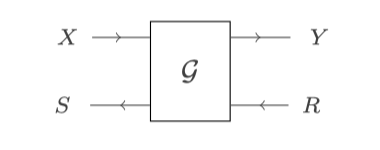
\includegraphics[width=0.5\linewidth]{images/GameSimple.png}
	\caption{A string diagram of an open game \label{figure:Fig. 10}}
	
\end{figure}

Putting this all together, we can refine the play function that takes a strategy as input, and returns a coend lens giving the execution of that strategy and a continuation giving some real-valued payoff. 

\begin{Definition} (Bayesian agent, from \cite[Definition 4.4.1]{BayesianOpenGames}) Let $S$, $A$ be sets. Then a Bayesian agent $G: (S,I) \rightarrow (A,B)$ is given by: 
	\begin{enumerate}
		\item A set of strategy profiles $\Sigma: X -> \Prob(A)$
		\item A play function $P : \Sigma \rightarrow \mathbf{CL}((X,S), (Y,R))$
		\item A best response function $B: X \times (Y \rightarrow R) \rightarrow Rel(\Sigma)$
	\end{enumerate}

\end{Definition}

A Bayesian agent corresponds to the open game given by the function \ensuremath{\Varid{dependentDecision}}, which restricts 

By precomposing a game that makes an observation with a copy operation (\cite[Definition 4.4.3]{BayesianOpenGames}), we give the rest of the model access to this observation (and its distribution). 

For example, 
this $\Theta$ may be some prior distribution representing an agent's belief of their type. Given a prior joint distribution $\Prob(\Theta \times S)$ where $\Theta$ is the unobservables and $S$ is the observable states, the agent can update this prior to a posterior and maximize their expected utility. 

This maximization is baked into the function \ensuremath{\Varid{dependentDecision}}, which generates an open game of a particular type. 
Starting to think of each of these open games as programs, an open game has four types associated with it. 
Here variables $X, Y$ are flowing covariantly (intuitively, flowing forwards) and $S, R$ are flowing contravariantly (which represent the feedback of information). Specifically: 
\begin{itemize}
	\item $X$ is the set of inputs that the open game can observe 
	\item $Y$ is the set of actions that the open game can take, or \textit{outcomes}
	\item $S$ is the set of \textit{co-outcomes} with the purpose of propagating information to precomposed games. 
	\item $R$ is the set of \textit{outcomes}
\end{itemize}

Note that there is no sense of agency attached to open games right off the bat. We have flexibility to define the behaviour of the open system according to our needs, whether as 
a representation of a utility-maximizing agent, or simply a function.  

The type of $\Sigma$, like a pure strategy profile in normal-form games, can be selecting an action from the set of actions. 
For sequential games, a strategy would typically involve choosing an action in response to each possible observed action played previously, 
thus such a strategy would be a function of type $X \rightarrow Y$.



\begin{hscode}\SaveRestoreHook
\column{B}{@{}>{\hspre}l<{\hspost}@{}}%
\column{4}{@{}>{\hspre}l<{\hspost}@{}}%
\column{E}{@{}>{\hspre}l<{\hspost}@{}}%
\>[B]{}\Varid{openGame}\;\Varid{var1}\;\Varid{var2}\mathrel{=}[\mskip1.5mu \Varid{opengame}\mid {}\<[E]%
\\
\>[B]{}\hsindent{4}{}\<[4]%
\>[4]{}\Varid{inputs}\mathbin{:};{}\<[E]%
\\
\>[B]{}\hsindent{4}{}\<[4]%
\>[4]{}\Varid{feedback}\mathbin{:};{}\<[E]%
\\
\>[B]{}\hsindent{4}{}\<[4]%
\>[4]{}\mathbin{:----------------------------:}{}\<[E]%
\\[\blanklineskip]%
\>[B]{}\hsindent{4}{}\<[4]%
\>[4]{}\Varid{inputs}\mathbin{:};{}\<[E]%
\\
\>[B]{}\hsindent{4}{}\<[4]%
\>[4]{}\Varid{feedback}\mathbin{:};{}\<[E]%
\\
\>[B]{}\hsindent{4}{}\<[4]%
\>[4]{}\Varid{operation}\mathbin{:};{}\<[E]%
\\
\>[B]{}\hsindent{4}{}\<[4]%
\>[4]{}\Varid{outputs}\mathbin{:};{}\<[E]%
\\
\>[B]{}\hsindent{4}{}\<[4]%
\>[4]{}\Varid{returns}\mathbin{:};{}\<[E]%
\\[\blanklineskip]%
\>[B]{}\hsindent{4}{}\<[4]%
\>[4]{}\mathbin{:----------------------------:}{}\<[E]%
\\[\blanklineskip]%
\>[B]{}\hsindent{4}{}\<[4]%
\>[4]{}\Varid{outputs}\mathbin{:};{}\<[E]%
\\
\>[B]{}\hsindent{4}{}\<[4]%
\>[4]{}\Varid{returns}\mathbin{:};{}\<[E]%
\\[\blanklineskip]%
\>[B]{}\mid \mskip1.5mu]{}\<[E]%
\ColumnHook
\end{hscode}\resethooks


\begin{enumerate}
   \item $X \rightarrow Y$
   \item $X \times R \rightarrow S$
\end{enumerate}

Breaking down the best response function, note othe domain $X \times \rightarrow$

\begin{definition}The category of open games, $\mathbf{Open}$
\end{definition}


Thus, we can begin thinking of an agent as defined by a) what it sees, b) what it does, c) what it sees according to the action it took. 
Departing from the standard of defining a global structure around agents, payoffs, and strategies, we can understand agents as a wider class of abstract notions called "open games." 
How we want these open games to be able to interact with each other can have well-defined properties as morphisms of a category. T
he objects of this category encode the data given in a), b), and c). 



As we see in the corresponding string diagram, the forward (or covariant) arrows correspond to \textit{inputs} and \textit{outputs}, and 

\textit{inputs}, as expected, is where to declare the input to the game. This is typically used  to define the state of a game, observed types or observed actions of other players. Note that declaring these as variables in this line brings them into scope for all other In a 2-player sequential game in the classical sense, the follower player observes the actions of the fi
Thus one way of "doing" compositional game theory can be done by drawing a string diagram to represent open games. 

As outlined in \cite{tan2022a} for designing institutions with a software 

\subsubsection{Contexts}


\section{Modularity in game theoretic cybersecurity modelling}
\label{sec:1}
\subsection{Overview}

The stark reality of designing effective cybersecurity games is bridging real-world security concerns with an accurate representation in a game-theoretic terms. Numerous models have been constructed and analyzed according to specific security problems, thus tying the models to their specification. Furthermore, these models often extend or adapt previously existing constructions by making new assumptions, using different payoff schemes, or integrating the model into an automated defensive infrastructure. Although this informal relationship between these models have been surveyed, there has yet to be a generalized framework for mechanizing this relationship as a standardized game formulation process. 

In this chapter, we examine a variety of security games and remark on similarities and differences between game-formulation methods. By identifying and encoding the commonly-used 2-player security game in the open-games-DSL, we show how to recover more complex models using this as a building block. By working in the open-games-DSL, a modeller can control information flow, introduce parallel subsystem security interactions, and reuse models. I review current security game analysis methods and present the possibility of integration with other tools. Finally, I propose an \textit{iterative development}-esque model generation process using the open-game engine.




%Indeed, the same code to analyze the intorduction of a single security interaction can analyze it in the context of a larger security infrastructure in a verifiable way.

%	 With an open-interfaced game representing a single security interaction, I demonstrate how a modeller can parameterize the game according to their security specification. 

%Finally, following
%The result of creating this representation is a game-theoretic model strictly tied to a security concern that is often encompassed by a larger security infrastructure. The system we may be trying to model is often comprised of subsystems. As attackers or defenders of this system we can think about an attack on the system as a whole or on its parts, or a mixture of both. 


 


% DOMAIN EXPERT

\subsection{Current state-of-the-art}
Using game theory to inform cybersecurity problems has seen growth in recent years with the development of a number of different models for evaluating Denial-of-Service attacks on cloud infrastructures, intrusion detection systems, and advanced persistent threats. Refer to the following surveys \cite{Pawlick2019}, \cite{Hausken2024}, \cite{Manshaei2013} for an overview of the wide collection of game-theoretic models. 

A general procedure for developing these models can be (roughly) summarized in the following steps: 
\begin{enumerate}
	\item Detail the security scenario and system, vectors of attack, and defensive capabilities
	\item Develop abstractions  and parameters for the players, actions, and payoff in a game-theoretic setting according to the security scenario
	\item Solve for a solution concept (i.e. Nash equilibrium, Subgame perfect Nash Equilibrium) using methods such as linear programming or Q-learning (for stochastic or repeated games)
	\item Deploy new strategies or technologies in the system according to the solution concept above
	\item Conduct simulations with a fixed strategy, determine the highest expected utility for players and evaluate system performance under these conditions
\end{enumerate}

However, the most recent concerns with evolving attacker threats and dynamic security situations requires more complex game-theoretic models. These games can be part of a larger automated defensive system to update defensive strategies in real time as part of a larger infrastructure such as in \cite{Jin2018}, \cite{Zhu2012}. The progression of these models often relies on the extension and variation of these game-theoretic models. For example, we may need to consider scalfing the number of players or repeating strategic interactions. The models presented in \cite{Chen2009}, \cite{Nochenson2012} suggest the use of the models as a basis for extensions and increased-complexity for other security scenarios. Similarly in \cite{Pawlick2015}, the signalling game structure are derived from \cite{Carroll2009}, with adjustments to the utilities. We'll see later how these models written in open games allow for easy extensionality.

According to \cite{Collins2025} evaluating 86 different game-theoretic models in cybersecurity, there already exists a sense of homogeneity between these models, where 76\% of models only cover a two-player security interaction, and 79\% use Nash (or variants of) equilibrium solution concepts for analysis. The authors also recommended a formal method for modellers to state their assumptions of the model that follow more in-line with cybersecurity concepts. Expanding on this idea in particular, we propose that code-based methods for stating assumptions allows for clear, testable specifications (see \ref{sec:2}). Only 24 or the 86 studies shown consider "multiple variants" of the constructed model. The specification of two criterion: (1) "Efficacy of Modelling" and (2) "Practicality of Solutions" serve as a framework for evaluating the tractability of game-theoretic models' representation of the underlying real cyber-interaction. The resulting recommendations are taken into account for the purposes of this thesis: 
\begin{enumerate}
	\item The need for a game space abstraction 
	\item Allow for more flexible assumptions
\end{enumerate}

In that same vein, \cite{Egan2025}, \cite{Liang2013} call for better scalability of models, in particular addressing models that account for more than two player games. Similarly, \cite{lye2005game} 
%\subsubsection{Qualitative to quantitiative parameterization}
%\cite{Rass2017}
%This necessitates collaboration between a domain expert (e.g. cybersecurity expert) and a game-theorist to translate sensible payoff schemes and parameters. 
%
%On the other hand, databases such as NIST and CSVV are directly used in \cite{MacQueen2020} \cite{Furuncu2015}. Diving deeper into \cite{Chen2009}, the work does not consider correlation between attack targets and leaves it for future work. The theoretical basis for the payoffs involving reputation, punishment for loss contrasts with other payoffs using server downtime or capital expenditure from NIST (CVSS) metrics. 

\subsubsection{Discussion on rational verification}
Rational verification is an approach to verifying the properties of multiagent systems where each agent is self-maximizing over some preference or utility. Inspired by classical model-checking paradigms, a specification is provided as a temporal logical formula describing a desired property of a multi-agent system. Then, the question is to verify whether a run (or simulation) of the system for some strategy profile is an equilibrium satisfying the property. Therefore, I consider open games as exactly the mechanism for expressively developing these systems with a built-in way to simulate behaviour. 

By using the PRISM-model checker and the PRISM property-specification language, it has been shown that security games can be mechanically verified. More recent work has extended PRISM to handle Stackelberg equilibrium for security games \cite{Phetmanee2024}. The complete software for two example models can be found at \cite{phetmanee_2024_13338608}. According to the proposed worfklow, there are automated tools to translate CVEs to attack-defense trees to Stackelberg Security Games, defined as a data structure storing the extensive-form representation of the game and atomic propositions that encode the reward structure as dictated in the attack-defense tree. For future work, encoding attack-defense trees defined in other models to be compatible with supplying payoffs in open games would be an interesting direction.

However, the models developed in \cite{Phetmanee2024} aren't built expressively for the reason of further extensionality in the future. The deliverable allows a user to provide a specific CVE and attacker action as a logical formula, and line-by-line entries for associated costs for specific attacker or defender actions. Finally, a security expert can input a certain patch or security property to test for Stackelberg equilibrium and whether that security property can be satisfied. 

The output of the StEve tool and the open-games diagnostic info are similar in terms of displaying each players associated payoff. However, the open-games-engine doesn't prove any satisfiability constraints, it's up to the modeller to check all possible states, whereas PRISM will be able to compute equilibrium automatically. Thus, StEve requires less understanding from security experts for running the game model, but prevents any amendments to game structure, such as an attacker being first-to-act rather than the defender. Working in the open-games environment necessitates more direct construction of the game with at most the import of the security games provided as a template in this thesis, but allows for greater maneuverability.

Comparatively, working in Haskell vs PRISM comes with the advantage of a type checker and various other language tools that will be expounded upon in the following chapter. An example difference is not needing to translate into a temporal logic formulae, but writing property tests using Hspec. The perceived downside is the inherent difference in computational complexity and running time for these models, which has yet to be determined. But from a useability point-of-view, a modeller can programmatically generate different attack or defense strategy profiles to test for any given model. 


\subsection{A first-attempt example}
In this section I'll detail a contrived example, as a first-pass to using the open-game-engine. I'll briefly cover how to interpret some of the fundamental parts of using the engine and understanding the diagnostic information provided in the output of an evaluation. I'll use code snippets to illustrate the thinking behind constructing each game, but I refer readers to the provided codebase for complete and executable models.

Breaking this down, we'll say the \textit{attackerDefenderGame} is a generic 2-player security game, in this case with the defender being able to observe the attacker's decision. We can represent a utility-maximizing attackers and defenders in code using the \textit{dependentDecision} function, which returns an open game. 

In games of \textit{incomplete information}, players have their own private types that are hidden from others. This is a common structure for security games, where a defender has to optimize their defensive strategies with uncertainty of the type of the adversary. This is a common structure used in Bayesian security games, typically by identifying behaviour of either an attacker or defender and their capabilities. In this case, the \textit{nature} game can be parameterized by a distribution over user-defined visitor types.  

As a modeller, I'm concerned with instantiating this interaction to my needs by supplying the required parameters given as arguments for \textit{attackerDefenderGame}. A well-researched optimization problem in cybersecurity is resolving a networks uncertainty about a user that has logged into the system, whether the user is a typical, honest user or an adversary \cite{}. The following details a way to instantiate this game with the arguments: 

\begin{enumerate}
	\item  \textit{distType} as a distribution \textit{distFromList[(User, 0.5), (Attacker, 0.5)]} to demonstrate a 50\% chance of encountering an attacker. \textit{distFromList} is a function that returns a distribution according to a list of tuples corresponding to the probability a certain type is drawn. 
	\item  \textit{actionSpaceAttacker} as a list \textit{[Access, NotAccess]} 
	\item \textit{actionSpaceDefender} as a list \textit{[Open, Close]}
\end{enumerate}

As with Bayesian security games, payoff behaviour is inherently tied to the types of the players. A simple hard-coded set of Haskell functions can be used to associate payoffs as \textit{Double} to be supplied to each player as \textit{attackerPayoff} and \textit{defenderPayoff}. Since there has to be a payoff for each possible outcome of the game, that would be exponential in the size of the action space of the model, in this case ${2^3}$ For defining payoffs, we can use a variety of sources but up to the discretion of the way we choose to model this encounter. In the commonly-used story-book style of describing this, we can say if the visitor is an attacker that attempts to access a server and the defender allows this access, the payoff is 100, which corresponds to a base payoff for a successful attack.

Thus this may be written as a Haskell function that pattern matches over each of these possibilities, partially written as: 

Thinking in a classical game theory style, this game can be represented as a balanced extensive form game tree, with sequentially-played subgames corresponding to each possible type doled out by the Nature player at the root node. Under each of the two types, the attacker can make two choices, and for each of these two choices, the defender can make two choices. As expected, each of the 8 leaves of the tree have the corresponding payoffs that would match the above payoff function.

Finally, given this payoff function (or more formally, a context to close the game), we would like to determine whether a strategy profile is included in the best-response relation generated by this model. Let's take a pure strategy profile such that the visitor always accesses regardless of type, and the defender opens access regardless of the visitor's choice. We can write these strategies as Kleisli arrows as follows: 


A straightforward to read the type signature of these strategies, assuming no previous knowledge of Kleisli arrows, is providing the \textit{Kleisli} constructor with a function that takes as input exactly what the player observes as input in their open game representation. In this case, for the attacker strategy, the "inputs" field is the \textit{visitorType}, so we need the attacker's corresponding strategy to have \textit{visitorType} as input. Similarly, the return type of the function we pass to the \textit{Kleisli} constructor almost exactly matches up with the "output" field of the open game, again for the attacker the type \textit{VisitorMove}. The only catch is that we're allowing for probabilistic choices as dictated by the \textit{Stochastic} type constructor, so we use the handy \textit{playDeterministically} helper function which wraps the value into this type, "playing" that value with probability 1. 

Now we have the bare ingredients to do some analysis on this game. The basic question we can now ask is, are these strategies for the attacker and defender a Nash Equilibrium? In other words, are the strategies such that no player is incentivized to unilaterally deviate their strategy? The current form of the diagnostics provided by the open-game-engine include payoffs given each player plays according to their supplied strategy, and the maximum possible payoff for another strategy. To put it more explicitly, each \textit{OpenGame} implements functionalities corresponds to the definitions in (\cite{HedgesThesis}, \cite{BayesianOpenGames}), as \textit{play} and \textit{evaluate}. 

\begin{enumerate}
	\item \textit{play} corresponds to the play function which takes a strategy as input, and returns an optic describing the behaviour of the game. 
	\item \textit{evaluate} encapsulates the best-response relation (or equilibrium function) found in open games literature, which takes a context and strategy as input, and determines whether that strategy profile is in the best-response set. 
\end{enumerate}





\subsection{Identifying compositional trends}
%Open games aren't necessarily a catch-all for solving any modelling problem, as briefly outlined in \cite{Hedges2019}. At risk of "overengineering" a problem (another term taken from software design), we'll first verify that the inherent structural similarities of preexisting models are already indicative of a need for a compositional approach. The following figure was inspired from a talk about "flexiformal mathematics" given by Michael Kohlhase at a kick-off meeting about applying LLMs for improving proof assistants, depicting the relationship between formality  and functionality. In the context of this thesis, we'll adapt this relationship such that we'll consider formality brought on by compositionality, hence the figure's depiction of the relationship between compositionality and functionality. 
We can begin to see some of the advantages of treating game-theoretic modelling in a compositional way: these functionalities are well-defined under the composite of games, so we can observe the behaviour of players relative to each other using the same infrastructure. The interchange of these analytics and how to separate the moving pieces to effectively compare and contrast models thus ends up as a problem of organizing this infrastructure. The following chapter will detail exactly how software-engineering principles exactly encapsulate this infrastructure. 




\begin{Definition}[2-player security game]
	A 2-player security game is a strategic interaction between two utility-maximizing agents dubbed \textit{attacker} and \textit{defender}, where an attacker seeks to access, gain control, or cause damage to a system, and a defender seeks to deploy countermeasures and prevent damage and intrusion.
\end{Definition}

This definition is made purposefully vague, with no indication of sequence of play or how exactly we quantify "seeks to ..." in our model. This will be our most general definition of security game, which we will  adapt according to our specification of the problem. This immediately begins to address the issue remarked by Liang in \cite{Liang2013}, which remarks on how rigid security models can be. 

\subsubsection{Model adaptation}
After reviewing the literature, I identified where compositionality would prove effective for generating these models using open games: 

\begin{enumerate}
	\item Characterizing an attacker and a defender as an open game
	\item Lifting 2-player attacker-defender interactions to a multiplayer, layered security scenario
\end{enumerate}

A prime example of model adaptation in literature is \cite{Pawlick2015} specifically adapts a signalling game from \cite{Carroll2009}, maintaining the same game structure and payoff scheme. 

\subsubsection{Subsystem specification}
Consider the architecture of a typical IDN as seen in Figure \ref{figure:Fig. 3}. This work formulates a two-layer stochastic, two-player game between an attacker and an IDN, where the states of the game are defined by the status of each subsystem. Here, the assumption is that the capabilities of each of the IDSs and their respective attackers as homogenous. In particular in the \textit{Simulation} section, the proposed model is evaluated with a specific set of parameters in a network of three IDSs and three independent attackers. It's self-evident that if the assumption of homogeneity was to change, the parameters used to evaluate the model must also change. Maintaining consistency across the model requires flexbility, but current game formulation techniques aren't necessarily built with the notion of seamless integration.

From a security design point-of-view, this interaction between subsystems is vital, especially if a vulnerability in one system affects the defensive capabilities of another. After designing games for a subsystem, we can easily direct the flow of the result of the game to a level-higher for resource management. In the typical style of "separation of concerns," designing these models using open games allows us to work on each subsystem separately from the aggregation mechanism. The disjoint nature of these parts allows for testing the efficacy of a different aggregation mechanisms or subsystems. 


\begin{figure}
	\centering
	
\includegraphics[width=0.5\linewidth]{IDNBlockDiagram.png}
	\caption{A block diagram for an IDN, for three subsystems from \cite{Jin2018} \label{figure:Fig. 3}}
	
\end{figure}

In order to run simulations using the constructed model formulation, the authors assigned values such as the detection libraries available to each IDS system $i$ and attacking libraries for each attacker $j$. \cite{He2015} 


The spirit of this thesis has certainly been explored in other work, for example in the simulation procedure provided by \cite{Nochenson2012}. This thesis attempts to mechanize the claims for "easily extendable" or "replace lines 9-13 in Algorithm 1" by providing a procedure that randomizes machine vulnerability values for each of 50.000 iterations, 

An iterative-style approach is further alluded to \cite{wellman2006methods}, a simulation-based approach to inform the general game-theoretic design process 

According to section 6.1 on IDS optimization in \cite{Collins2025}, there is a recommendation for characterizing and distinguishing different kinds of attackers and varying objectives.  

\subsection{Constructing an iterative design process}
\subsubsection{Addressing the ad-hoc design process}
Many game-theoretic models in security rely on ad-hoc schemes \cite{Liang2013}. The authors also cite a need for standards for designing payoffs and more scalable methods to match the complexity of the security problem, such as building a model that considers more than three players. The cybersecurity problem specifications dictate the parameters and format of the model, creating a hyper-focused game. So translating the real-world security situation to a model using the same toolbox of game-theoretic mechanisms implies the need for the right sandbox to test different real-world translations and how they respond in the game-theoretic model. 

%Therefore, we need to develop abstractions that allow for systematic instantiation of game-theoretic models according to \textit{many} of these real-world translations. 
The work conducted in \cite{Caulfield2015}, \cite{Caulfield2014} closely resembles compositional and software-supported approach in security modelling by \textit{a priori} designing models that can be composed together later. Here the authors present a systems modelling theory for security policy design. Using a semantic-approach based on process theories to model elements of a security situation as resources of these theories, these concepts can be encoded in Julia to run simulations. They show composition of models is well-defined and demonstrate how to run these models based on individual expected utility. The result is a model to help inform security policy managers make better decisions about security systems and have a framework to convey this information to other stakeholders.  

This modelling approach is focused on the security of an organization comprised of three sequentially-composable models: (1) a device-loss model, (2) a tailgating model, and (3) a document-sharing model. The pitch most strongly reminiscent to this thesis is that a modeller can adaptively see how including or excluding elements of a model to the workflow affects the system in a reactive way. For example, the modeller can examine the simulated data of just the tailgate model with and without the presence of a security guard on the frequency of computer accesses, and then observe the impact of the same presence of a security guard in the large composed model. This layered approach of designing locations and resources on a layer under the decision-making layer of agents hints at a design approach that separates the concerns of the model from its instantiation. This thesis tackles a different class of security problems but mirrors the task of formalizing security problems in a compositional and iterative way.

Furthermore, an iterative, formalized process for refining games is not new. In particular, \textit{empirical game-theoretic analysis} is a methodology that learns payoff profiles and strategy spaces through simulated data to inform the game formulation. Specifically, the goal is to instantiate an empirical game which is parameterized by simulating expected payoffs according to a strategy profile. Two feedback mechanisms are leveraged: (1) payoff estimation and (2) strategy space exploration.  This methodology has seen its applicability in moving target defense \cite{Wellman2015} and adaptive cyber defense \cite{Wellman2019}. Further extensions for a software-induced workflow, including database support and use of Gambit, can be found in \cite{EGTAOnline}. \ref{figure:Fig. 2} provides a pipeline for generating these games. 

\begin{figure}
	\begin{center}
		
\includegraphics[width=0.5\linewidth]{EmpiricalAnalysisPipeline.png}
		\caption{A general modelling process from \cite{Wellman2015} \label{figure:Fig. 2}}
		
	\end{center}
\end{figure}

\begin{figure}
	\centering
	
\includegraphics[width=0.5\linewidth]{EGTAFeedback.png}
	\caption{Empirical game-theoretic analysis pipeline from \cite{Wellman2019} \label{figure:Fig. 3}}
\end{figure}

%The modelling methodology that will be proposed in this thesis follow more closely to \cite{Nochenson2012} and \cite{sengupta2017game}. 
%\subsection{Towards generating libraries for security models}
%An ancillary benefit of using a methodology insisting on flexible, open-interfaces is self-documenting, executable models for reuse later. 
%\subsubsection{Empirical approach to designing utility functions}
%For Bayesian security games, payoffs can be associated with types assigned to each player. 
%\subsubsection{Empirical approach to designing strategies}







\subsubsection{Proposed design methodology}
After conducting these translations and adaptations from pre-existing models in literature, it was clear that there were ways to improve how these models interacted or organizing the same code i.e. DRY ("don't repeat yourself"). A methodology to promote greater synergy between the initial conception of a security problem to it's game-theoretic translation is needed. 
\begin{enumerate}
	\item High-level model specification
	\item Game structure as an open game 
	\item Designing payoffs according to model specification
\end{enumerate}

\subsubsection{High-level model specification}
To begin the formulation process, a modeller identifies the specifications of the problem. We dub this "high-level" as a way of top-down identifying system-level and exogenous parameters relevant to the problem. The objectives of this stage are summarized as: 
\begin{enumerate}
	\item Identify players (attackers and defenders)
	\item Quantify action spaces and encode as Haskell data types
	\item Encode relevant system parameters as a Haskell data type
\end{enumerate}

At this point, a modeller may be asking questions such as "is equilibrium reached under this system configuration." Writing the bare-minimum code as per the usual test-driven development paradigm, we can write an identity open game parameterized by these exogenous parameters, verify the test passes, and continue. We'll see in the next chapter how Hspec has a nice tradeoff of writing human-readable specifications, and how to implement \textit{Gen} for these parameters to generate random test-cases for property-based tests. 

\subsubsection{Game-level specifications}
One level lower, we can consider game-level specifications, or in other words, the variables we consider directly in the game. These consist of action spaces in the usual sense, in this workflow as a list of data types. Constructively speaking, we first fix our exogenous parameters, then we fix the game-level parameters which characterize each player's capabilities.
 

% \tikzstyle{startstop} = [rectangle, rounded corners, 
% minimum width=3cm, 
% minimum height=1cm,
% text centered, 
% draw=black, 
% fill=red!30]

% \tikzstyle{io} = [trapezium, 
% trapezium stretches=true, % A later addition
% trapezium left angle=70, 
% trapezium right angle=110, 
% minimum width=3cm, 
% minimum height=1cm, text centered, 
% draw=black, fill=blue!30]

% \tikzstyle{process} = [rectangle, 
% minimum width=3cm, 
% minimum height=1cm, 
% text centered, 
% text width=3cm, 
% draw=black, 
% fill=orange!30]

% \tikzstyle{decision} = [diamond, 
% minimum width=3cm, 
% minimum height=1cm, 
% text centered, 
% draw=black, 
% fill=green!30]
% \tikzstyle{arrow} = [thick,->,>=stealth]
% \begin{figure}
% 	\centering
% 	\begin{tikzpicture}[node distance=2cm]
		
% 		\node (start) [startstop] {Security specification};
% 		\node (game) [startstop, below of=start] {Game specification};
% 		\node (pro1) [process, below of=game] {Process 1};
% 		\node (dec1) [decision, below of=pro1, yshift=-0.5cm] {Decision 1};
		
% 		\node (pro2a) [process, below of=dec1, yshift=-0.5cm] {Process 2a
% 			text text text text
% 			text text text 
% 			text text text};
		
% 		\node (pro2b) [process, right of=dec1, xshift=2cm] {Process 2b};
% 		\node (out1) [io, below of=pro2a] {Output};
% 		\node (stop) [startstop, below of=out1] {Stop};
		
% 		\draw [arrow] (start) -- (game);
% 		\draw [arrow] (game) -- (pro1);
% 		\draw [arrow] (pro1) -- (dec1);
% 		\draw [arrow] (dec1) -- node[anchor=east] {yes} (pro2a);
% 		\draw [arrow] (dec1) -- node[anchor=south] {no} (pro2b);
% 		\draw [arrow] (pro2b) |- (pro1);
% 		\draw [arrow] (pro2a) -- (out1);
% 		\draw [arrow] (out1) -- (stop);
		
% 	\end{tikzpicture}
% 		\caption{The proposed workflow}
% \end{figure}


\section{Software abstractions for open cybersecurity games}
\label{sec:2}
\subsection{Overview}
The previous chapter identified compositional patterns amongst a series of related game theoretic models for cybersecurity problems. But the process for analyzing the behaviour of the model requires additional work, specifically as the model increases in complexity. 

In this chapter, we show how to use the Haskell environment to generate parameters and specify the parameter space of games. Therefore, after using the DSL to con

There are many computational tools that exist in order to solve for equilibria, produce extensive-form game-trees, and SMT-solvers. But what we would like to outline in this chapter is being able to simultaneously generate games in a declarative manner, where the game formulation process is aided by the open games Haskell DSL. In this chapter we'll see how after a few attempts, generalizing these patterns allow for model \textit{reproducability} and \textit{reusability}, ultimately culminating in a small library of 2-player security games. We will see how this simple subset of game scan be used to rapidly generate game theoretic models in a variety of settings. By leveraging abstract data types, polymorphism, and the reader monad, we can parameterize these models with modules that help organize payoff modules and strategies. 

Providing a small subset of games as a library, this falls short of a clear-cut executable script for a predetermined model. Part of developing or extending a model could be better 



\subsection{Current state-of-the-art for open games}
This thesis draws on a key motivation proposed by Zahn in \cite{ZahnCybercat}, towards the synthesis of an encoded library of microeconomic models. The process of developing the "correct" model is therefore framed as a software engineering problem. The open-games-engine has demonstrated its use verifying the most recognizable game theory problems like Prisoner's Dilemma, to auction mechanisms. A series of these models have been met with production-level directions, and a codebase of models have grown. While this thesis departs from the application of this field towards cybersecurity, the bulk of the work that is presented here is an attempt to give guidelines for using the open-games-engine effectively. Specifically, the interdisciplinary and workflow possibilities that are provided by producing models in this environment, achieving easy maneuverability and testing that fits naturally with the requirements for synthesizing effective security models. 

\cite{20squares} has a series of completed projects for auctions and blockchain staking protocols. Capturing the complexity of models with open games is shown in these previous projects, but this chapter will deliberate on formalizing common techniques used to generate these models. I invite readers to refer to the README for \cite{20squares} projects for the syntax of the open-games DSL and common operators that can be used. 

\subsection{Formalizing Stackelberg equilibrium in open games}

\subsubsection{Related work}
The most recent work that uses software-assisted tools for Stackelberg security games is \cite{Phetmanee2024}, using rational verification. Rational verification is a formal-analysis technique for determining the equilibrium properties of multiagent systems. Specifically by encoding these properties in Linear Temporal Logic, practitioners can use model-checkers such as PRISM to verify that given models satisfy properties. After writing these propositions, PRISM can act as an equilibrium checker by checking all possible states of the game. In particular, \cite{Phetmanee2024} extends the PRISM framework to demonstrate the security properties detailed in CVE-2017-8759, and generates data demonstrating the defensive conditions and recommendations for security advisors. 

This thesis seeks to bring the resultant model closer to its conception, or in other words, more reactive to changes made to the original parameters of its conception. In the StEvE methodology, security experts are tasked with encoding an ADT and the corresponding payoffs, to then be encoded into the temporal logic propositions. A PRISM script can then ingest the CVE data and in-lined cost values to get an evaluation outputted to the terminal with metrics such as payoffs for attackers and defenders in each state.


\subsection{Model instantiation}
Drawing from the habit of separation-of-concerns, 
\subsection{Towards test-driven modelling}
Test-driven development (TDD) is a coding paradigm where a programmer begins with unit tests and iteratively refactors code to fulfill these tests and write new ones. A programmer doesn't move on to the next iteration until the entire test suite passes, ensuring that refactors don't cause breaking changes across a code-base. The very first test case in any situation is to verify the most basic assumptions for the behaviour of a program. And as the complexity and dependency of this program grows, these assumptions are always kept in check. TDD enables the coder to think about specifications first, and while those specifications are open to change over time, writing these tests document the expected behaviour of the program. 

Here I propose test-driven modelling as a way to guide experiments in a self-documented fashion, while also maintaining guarantees of a game before its eventual composition with others. 

It's a well-known fact that in the problem of a player allocating finite defensive resources across a series of subsystems, for example by employing maximum, high-cost 


\subsubsection{Generating test cases}

\subsection{Leveraging the Haskell type system}
\label{sec: types}
Type inference is a powerful tool for checking correctness of your models. And as a developer we can let the language work for us by observing a basic requirement for our model: type correctness. According to the proposed methodology, perhaps I've written that my specification as type sfor inputs and outputs for my attacker. Then to simulate the behaviour of the attacker, I need to supply the expected behaviour as a strategy where the attacker observes the expected input type and returns the expected output type. With these bounds in place, it leaves room for me to specify behaviour according to a wide variety of attack vectors or capabilities. 
\begin{enumerate}
	\item What the agent observes
	\item What the agent can do about it 
	\item All the 
\end{enumerate}


Working with the open-games DSL allows us to structure our game in a block-by-block style, however some of the major components of the model require Haskell functions to encode payoff matrices, action spaces

Definition: an open-game allows for attachments. As soon as we provide the associated payoff for the building block, we close off an end. So for each complete model, the agents: 


Parameters and hardcoded values: we often want to encode our behaviour as Haskell functions. For example, the level of defense may be dependent on the level of honeypot, and ... Often we need to keep track of constraints associated with these, which intuitively follows a specification written in QuickCheck. Following the specification, we can verify that we capture the expected behaviour with these functional tests 

The added benefit of generating test parameters and ensuring variable constraints are met.

The type checker will ensure that closing a game with a given payoff builder will mean that types must line up at the interfaces. 

\subsection{A few SOLID principles}
Open for extension ,closed for modification. The hallmark of this design strategy . Just as we might want to consider an additional player, we can easily replicate a utility-maximizing agent using the DSL. Similarly, if we would like to consider an additoinal model parameter or 

Having a modular language allows us to construct games open for extension, by interacting with the interfaces exposed by each game. 

IDEA: We want to encode our "assumptions" such as paraemter bounds, sign, and relative values. We cna quickcheck these as part of the simulation process in order to preliminarily check that test parameters used for simulation accurately reflect the given values. 
\subsubsection{Separation of concerns}

\subsection{Designing payoffs}
Based on examples provided in \cite{Zahn2024}, some of the following design patterns can be recognized:
\begin{enumerate}
	\item Type-specified payoffs 
	\item State-specified payoffs
\end{enumerate}
\subsubsection{Payoff parameterization with the reader monad}

\textbf{Goal:} the development of payoff modules that can be interchanged for a particular game.

Note that from section \ref{sec: types}, the instantiation of games by action space informs the types exactly available for designing payoffs. Since this model doesn't 'require' any specific payoff behaviour beyond these types (and passing some test infrastructure). We can loosely characterize payoff functions by their dependence on the following information: 
\begin{enumerate}
	\item The output of the designed game 
	\item Model-level exogenous parameters 
\end{enumerate}

An example of 1. in a simple case is a tuple of actions chosen by each player in the game, or the assigned player type. 2. is concerned with system parameters that are relevant to payoff data. Here, we propose the reader monad as the necessary function-passing structure for generating payoff functions according to these model-level exogenous parameters. 

\begin{hscode}\SaveRestoreHook
\column{B}{@{}>{\hspre}l<{\hspost}@{}}%
\column{E}{@{}>{\hspre}l<{\hspost}@{}}%
\>[B]{}\color{datatype}\texttt{type}\;\Conid{PayoffReader}\;\Varid{a}\mathrel{=}\Conid{Reader}\;\Varid{a}\;\Conid{Double}{}\<[E]%
\\[\blanklineskip]%
\>[B]{}\Varid{runPayoff}\mathbin{::}\Varid{a}\to \Conid{PayoffReader}\;\Varid{a}\to \Conid{Double}{}\<[E]%
\\
\>[B]{}\Varid{runPayoff}\;\Varid{params}\;\Varid{reader}\mathrel{=}\Varid{runReader}\;\Varid{reader}\;\Varid{params}{}\<[E]%
\ColumnHook
\end{hscode}\resethooks




Notice the parametric type \textit{a}, so we can define a \textit{PayoffReader} for any ADT containing exogenous model parameters. This supports the system-level-first architecture that allows a modeller to introduce relevant variables that are not directly involved and subject to manipulation separate from the interworkings of the open game model. Thus, we can actively test how different payoff schemes affect our game model, either by (1) testing the same game with different system variables or (2) the same system variables with different player capabilities. We can characterize a payoff profile's dependence on two things: the outputs of the open game, and the variables accessible with the \textit{PayoffReader}.

To start with writing payoffs according to the outputs of a game, we can consider the running Bayesian security game example from the previous chapter. Already we can consider branching the payoff functions into helpers associated with each type of player, and pattern-match on these types. If we use the preset template from the Security module, the set of two-player security games requires a \textit{PayoffReader} for each attacker and defender. Then at the execution-level of the game, which runs against the model-level parameters, we use these parameters to instantiate the readers (in this case, \textit{IDSParams}). Thanks to the type-checker, the output type of the model should provide the modeller with the requirements for this \textit{PayoffReader} constructor. In this example, we can define the payoffs as follows: 

% \begin{hscode}\SaveRestoreHook
% 	\column{B}{@{}>{\hspre}l<{\hspost}@{}}%
% 	\column{5}{@{}>{\hspre}l<{\hspost}@{}}%
% 	\column{14}{@{}>{\hspre}l<{\hspost}@{}}%
% 	\column{E}{@{}>{\hspre}l<{\hspost}@{}}%
% 	\>[B]{}\Varid{visitorPayoff}\mathbin{::}\Conid{VisitorType}\to \Conid{VisitorMove}\to \Conid{DefenderMove}\to \Conid{PayoffReader}\;\Conid{IDSParams}{}\<[E]%
% 	\\
% 	\>[B]{}\Varid{visitorPayoff}\mathrel{=}\lambda \mathbf{case}\;\{\mskip1.5mu {}\<[E]%
% 	\\
% 	\>[B]{}\hsindent{5}{}\<[5]%
% 	\>[5]{}\Conid{Attacker}\to \Varid{attackerPayoff};{}\<[E]%
% 	\\
% 	\>[B]{}\hsindent{5}{}\<[5]%
% 	\>[5]{}\Conid{User}\to {}\<[14]%
% 	\>[14]{}\Varid{userPayoff}{}\<[E]%
% 	\\
% 	\>[B]{}\mskip1.5mu\}{}\<[E]%
% 	\\[\blanklineskip]%
% 	\>[B]{}\Varid{defenderPayoff}\mathbin{::}\Conid{VisitorType}\to \Conid{VisitorMove}\to \Conid{DefenderMove}\to \Conid{PayoffReader}\;\Conid{IDSParams}{}\<[E]%
% 	\\
% 	\>[B]{}\Varid{defenderPayoff}\mathrel{=}\lambda \mathbf{case}\;\{\mskip1.5mu {}\<[E]%
% 	\\
% 	\>[B]{}\hsindent{5}{}\<[5]%
% 	\>[5]{}\Conid{Attacker}\to \Varid{defenderUnderAttackPayoff};{}\<[E]%
% 	\\
% 	\>[B]{}\hsindent{5}{}\<[5]%
% 	\>[5]{}\Conid{User}\to \Varid{defenderNormalPayoff};{}\<[E]%
% 	\\
% 	\>[B]{}\mskip1.5mu\}{}\<[E]%
% 	\ColumnHook
% \end{hscode}\resethooks

The type signature of each of these functions corresponds to the output of the completed open game. Then, we can use helper functions associated with each matched type and define the payoff accordingly. Since we've instantiated the reader with our exogenous parameters, the bottom-level of our payoff functions have access to the data of \textit{IDSParams}. Refer to \textbf{IDS/IDSAPayoff.hs} for the complete implementation.

A key feature of using the reader monad is having fine-tuned control over these parameters without worrying about changing them. And if we do need to change them, it's explicit. Consider the payoff scheme used to slightly adapt the previous example by allowing the defender to not just open or close, but deploy two different kinds of honeypots or remain open under normal operation in \textbf{IDS/IDSAHPPayoff.hs}, 

% \begin{hscode}\SaveRestoreHook
% 	\column{B}{@{}>{\hspre}l<{\hspost}@{}}%
% 	\column{5}{@{}>{\hspre}l<{\hspost}@{}}%
% 	\column{14}{@{}>{\hspre}l<{\hspost}@{}}%
% 	\column{E}{@{}>{\hspre}l<{\hspost}@{}}%
% 	\>[B]{}\Varid{defenderPayoffHP}\mathbin{::}\Conid{VisitorType}\to \Conid{VisitorMove}\to \Conid{HoneypotDeploymentMove}\to \Conid{PayoffReader}\;\Conid{IDSParams}{}\<[E]%
% 	\ColumnHook
% \end{hscode}\resethooks

The type signature only differs in the third argument to the payoff functions. Intuitively, I will have to write the same pattern-matching structure but over the new datatype \textit{HoneypotDeploymentMove}, but the computation of payoff shouldn't have to be rewritten explicitly. Since in my model, deploying a high-interaction honeypot increases the probability of detecting an adversary, this can be reflected by locally altering the \textit{IDSParams} before using the same formula from IDSAPayoff. So given a \textit{HoneypotDeploymentMove}, I want to update my \textit{PayoffReader} with an augmentation function such as: 

% \begin{hscode}\SaveRestoreHook
% 	\column{B}{@{}>{\hspre}l<{\hspost}@{}}%
% 	\column{E}{@{}>{\hspre}l<{\hspost}@{}}%
% 	\>[B]{}\Varid{augmentDetectionProb}\mathbin{::}\Conid{HoneypotDeploymentMove}\to (\Conid{PayoffReader}\;\Conid{IDSParams}\to \Conid{PayoffReader}\;\Conid{IDSParams}){}\<[E]%
% 	\\
% 	\>[B]{}\Varid{augmentDetectionProb}\;\Conid{HighInteractionHP}\mathrel{=}\Varid{local}\;(\lambda \Varid{params}\to \Varid{params}\;\{\mskip1.5mu \Varid{probDetected}\mathrel{=}\Varid{probDetected}\;\Varid{params}\mathbin{*}\mathrm{1.4}\mskip1.5mu\}){}\<[E]%
% 	\\
% 	\>[B]{}\Varid{augmentDetectionProb}\;\Conid{LowInteractionHP}\mathrel{=}\Varid{local}\;(\lambda \Varid{params}\to \Varid{params}\;\{\mskip1.5mu \Varid{probDetected}\mathrel{=}\Varid{probDetected}\;\Varid{params}\mathbin{*}\mathrm{1.25}\mskip1.5mu\}){}\<[E]%
% 	\\
% 	\>[B]{}\Varid{augmentDetectionProb}\;\Conid{Normal}\mathrel{=}\Varid{id}{}\<[E]%
% 	\ColumnHook
% \end{hscode}\resethooks



To demonstrate the breadth of this granularity, we observe the following example for designing payoffs derived from an initial problem statement.

\begin{enumerate}
	\item Assumption: there is only one attacker and one defender
	\item Assumption: the defender can either allow traffic or close the server 
\end{enumerate}

The factors that we consider that dictates the payoff would be included in the global config instantiating the model as a Haskell record type. Here, without having to change this global config, I use \textit{local} to adjust the detection probability. 


\subsubsection{Repeated payoff game structures}
As elaborated in \cite{Hedges2019}, we can introduce infinitely-repeated games by conditioning an open game according to some set we'll denote \textit{A}. For our purposes, we can consider conditioning a game by all the possible outcomes played in a stage game, whilst discounting the payoffs at each stage by some $\alpha$. 

Notice in the following definition of this repeated stage, besides the usual name and action space parameterization for each player the final argument is itself another open game dubbed \textit{payoffGame}. We can think about \textit{repeatedStage} as an open game with the sole purpose of accumulating passed back payoffs and sending them back to the next iteration in the \textbf{feedback} field. Here we set the \textit{feedback} and \textit{returns} types as a list of Doubles of length two for the two-player security game case. 
\begin{hscode}\SaveRestoreHook
\column{B}{@{}>{\hspre}l<{\hspost}@{}}%
\column{4}{@{}>{\hspre}l<{\hspost}@{}}%
\column{11}{@{}>{\hspre}l<{\hspost}@{}}%
\column{E}{@{}>{\hspre}l<{\hspost}@{}}%
\>[B]{}\Varid{repeatedStage}\;\Varid{actionSpaceAttacker}\;\Varid{attackerName}\;\Varid{actionSpaceDefender}\;\Varid{defenderName}\;\Varid{payoffGame}\mathrel{=}[\mskip1.5mu \Varid{opengame}\mid {}\<[E]%
\\
\>[B]{}\hsindent{4}{}\<[4]%
\>[4]{}\Varid{inputs}\mathbin{:}\Varid{visitorType},\Varid{prevAttackerDecision},\Varid{prevDefenderDecision};{}\<[E]%
\\
\>[B]{}\hsindent{4}{}\<[4]%
\>[4]{}\Varid{feedback}\mathbin{:}[\mskip1.5mu (\Varid{payoffIndexer}\;\Varid{previousPayoffs}\;\mathrm{0})\mathbin{+}\Varid{attackerPayoff},(\Varid{payoffIndexer}\;\Varid{previousPayoffs}\;\mathrm{1})\mathbin{+}\Varid{defenderPayoff}\mskip1.5mu];{}\<[E]%
\\
\>[B]{}\hsindent{4}{}\<[4]%
\>[4]{}\mathbin{:----------------------------:}{}\<[E]%
\\[\blanklineskip]%
\>[B]{}\hsindent{4}{}\<[4]%
\>[4]{}\Varid{inputs}\mathbin{:}\Varid{visitorType},\Varid{prevAttackerDecision},\Varid{prevDefenderDecision};{}\<[E]%
\\
\>[B]{}\hsindent{4}{}\<[4]%
\>[4]{}\Varid{feedback}\mathbin{:};{}\<[E]%
\\
\>[B]{}\hsindent{4}{}\<[4]%
\>[4]{}\Varid{operation}\mathbin{:}\Varid{attackerLeader}\;\Varid{attackerName}\;\Varid{actionSpaceAttacker};{}\<[E]%
\\
\>[B]{}\hsindent{4}{}\<[4]%
\>[4]{}\Varid{outputs}\mathbin{:}\Varid{attackerDecision};{}\<[E]%
\\
\>[B]{}\hsindent{4}{}\<[4]%
\>[4]{}\Varid{returns}\mathbin{:}(\Varid{payoffIndexer}\;\Varid{previousPayoffs}\;\mathrm{0})\mathbin{+}\Varid{attackerPayoff};{}\<[E]%
\\[\blanklineskip]%
\>[B]{}\hsindent{4}{}\<[4]%
\>[4]{}\Varid{inputs}\mathbin{:}\Varid{prevAttackerDecision},\Varid{prevDefenderDecision};{}\<[E]%
\\
\>[B]{}\hsindent{4}{}\<[4]%
\>[4]{}\Varid{feedback}\mathbin{:};{}\<[E]%
\\
\>[B]{}\hsindent{4}{}\<[4]%
\>[4]{}\Varid{operation}\mathbin{:}\Varid{defenderFollower}\;\Varid{defenderName}\;\Varid{actionSpaceDefender};{}\<[E]%
\\
\>[B]{}\hsindent{4}{}\<[4]%
\>[4]{}\Varid{outputs}\mathbin{:}\Varid{defenderDecision};{}\<[E]%
\\
\>[B]{}\hsindent{4}{}\<[4]%
\>[4]{}\Varid{returns}\mathbin{:}(\Varid{payoffIndexer}\;\Varid{previousPayoffs}\;\mathrm{1})\mathbin{+}\Varid{defenderPayoff};{}\<[E]%
\\[\blanklineskip]%
\>[B]{}\hsindent{4}{}\<[4]%
\>[4]{}\Varid{inputs}\mathbin{:}\Varid{visitorType},\Varid{attackerDecision},\Varid{defenderDecision};{}\<[E]%
\\
\>[B]{}\hsindent{4}{}\<[4]%
\>[4]{}\Varid{feedback}\mathbin{:};{}\<[E]%
\\
\>[B]{}\hsindent{4}{}\<[4]%
\>[4]{}\Varid{operation}\mathbin{:}\Varid{payoffGame};{}\<[E]%
\\
\>[B]{}\hsindent{4}{}\<[4]%
\>[4]{}\Varid{outputs}\mathbin{:}\Varid{attackerPayoff},\Varid{defenderPayoff};{}\<[E]%
\\
\>[B]{}\hsindent{4}{}\<[4]%
\>[4]{}\Varid{returns}\mathbin{:};{}\<[E]%
\\
\>[B]{}\hsindent{4}{}\<[4]%
\>[4]{}\mathbin{:----------------------------:}{}\<[E]%
\\[\blanklineskip]%
\>[B]{}\hsindent{4}{}\<[4]%
\>[4]{}\Varid{outputs}\mathbin{:}\Varid{visitorType},\Varid{attackerDecision},\Varid{defenderDecision};{}\<[E]%
\\
\>[B]{}\hsindent{4}{}\<[4]%
\>[4]{}\Varid{returns}\mathbin{:}\Varid{previousPayoffs};{}\<[E]%
\\
\>[B]{}\mid \mskip1.5mu]{}\<[E]%
\\[\blanklineskip]%
\>[B]{}\Varid{repeatedPayoffGame}\;\Varid{params}\;\Varid{payoffReader1}\;\Varid{payoffReader2}\mathrel{=}[\mskip1.5mu \Varid{opengame}\mid {}\<[E]%
\\
\>[B]{}\hsindent{4}{}\<[4]%
\>[4]{}\Varid{inputs}\mathbin{:}\Varid{visitorType},\Varid{prevAttackerDecision},\Varid{prevDefenderDecision};{}\<[E]%
\\
\>[B]{}\hsindent{4}{}\<[4]%
\>[4]{}\Varid{feedback}\mathbin{:};{}\<[E]%
\\
\>[B]{}\hsindent{4}{}\<[4]%
\>[4]{}\mathbin{:----------------------------:}{}\<[E]%
\\[\blanklineskip]%
\>[B]{}\hsindent{4}{}\<[4]%
\>[4]{}\Varid{inputs}\mathbin{:}\Varid{visitorType},\Varid{prevAttackerDecision},\Varid{prevDefenderDecision};{}\<[E]%
\\
\>[B]{}\hsindent{4}{}\<[4]%
\>[4]{}\Varid{feedback}\mathbin{:};{}\<[E]%
\\
\>[B]{}\hsindent{4}{}\<[4]%
\>[4]{}\Varid{operation}\mathbin{:}\Varid{liftStochastic}\;(\lambda (\Varid{x},\Varid{y},\Varid{z})\to \Varid{playDeterministically}\;(\Varid{calculateCurrAttackerPayoff}\;\Varid{x}\;\Varid{y}\;\Varid{z},\Varid{calculateCurrDefenderPayoff}\;\Varid{x}\;\Varid{y}\;\Varid{z}));{}\<[E]%
\\
\>[B]{}\hsindent{4}{}\<[4]%
\>[4]{}\Varid{outputs}\mathbin{:}\Varid{payoff1},\Varid{payoff2};{}\<[E]%
\\
\>[B]{}\hsindent{4}{}\<[4]%
\>[4]{}\Varid{returns}\mathbin{:};{}\<[E]%
\\[\blanklineskip]%
\>[B]{}\hsindent{4}{}\<[4]%
\>[4]{}\mathbin{:----------------------------:}{}\<[E]%
\\[\blanklineskip]%
\>[B]{}\hsindent{4}{}\<[4]%
\>[4]{}\Varid{outputs}\mathbin{:}\Varid{payoff1},\Varid{payoff2};{}\<[E]%
\\
\>[B]{}\hsindent{4}{}\<[4]%
\>[4]{}\Varid{returns}\mathbin{:};{}\<[E]%
\\[\blanklineskip]%
\>[B]{}\mid \mskip1.5mu]\;\color{datatype}\texttt{where}\;\Varid{calculateCurrAttackerPayoff}\;\Varid{x}\;\Varid{y}\;\Varid{z}\mathrel{=}\Varid{runPayoff}\;\Varid{params}\;(\Varid{payoffReader1}\;\Varid{x}\;\Varid{y}\;\Varid{z}){}\<[E]%
\\
\>[B]{}\hsindent{11}{}\<[11]%
\>[11]{}\Varid{calculateCurrDefenderPayoff}\;\Varid{x}\;\Varid{y}\;\Varid{z}\mathrel{=}\Varid{runPayoff}\;\Varid{params}\;(\Varid{payoffReader2}\;\Varid{x}\;\Varid{y}\;\Varid{z}){}\<[E]%
\ColumnHook
\end{hscode}\resethooks
\subsection{Collaboration}
To conceptualize the game requires a translation of the security situation to the game-theoretic situation. Whether we choose tractable solutions like payoffs corresponding to server up-time, there is a need for some system in order to communicate this information. Furthermore, specifications... As demonstrated, we would like reproducability and modularity to rapidly provide analytics according to specifications. (SOURCE CONTROL)

%--------------------------------
% Bibliography
%--------------------------------
\clearpage
\setstretch{1.0}  % 1.0 line spacing. 
\printbibliography
\clearpage

%--------------------------------
% Appendices
%--------------------------------
%\appendix
\setstretch{1.5} % 1.5 line spacing.
%\section{Appendix}
\lipsum[1-2]
\subsection{A subsection}
\lipsum[1-2]
\subsubsection{A subsubsection}
\lipsum[1-2] % Add one file per appendix

\end{document}
